\documentclass[11pt,a4paper]{article}
\usepackage[margin=1in]{geometry}
\usepackage{amsmath,amssymb}
\usepackage{booktabs,longtable,array}
\usepackage{graphicx}
\usepackage{hyperref}
\usepackage{natbib}
\usepackage{caption}
\usepackage{subcaption}
\usepackage[disable]{microtype}
\usepackage{xcolor}
\hypersetup{colorlinks=true,linkcolor=blue,citecolor=blue,urlcolor=blue}

\newcommand{\Hmin}{H_{\min}}
\newcommand{\Ascore}{A}
\newcommand{\kB}{k_{\mathrm{B}}}
\newcommand{\Tbody}{T_{\mathrm{body}}}

\title{The Thermodynamic Floor of Vertebrate Cellular Identity:\\
Methylation Entropy, Body Temperature, and Maximum Lifespan\\
across 500 Million Years of Evolution}

\author{Heath W.\ Mahaffey\\
\small Independent Researcher, Entiat WA\\
\small \href{mailto:hmahaffeyges@gmail.com}{hmahaffeyges@gmail.com}\\
\small \href{https://iamperformance.net}{iamperformance.net}\\[4pt]
\small Provisional Patents: US~64/012,720 \& US~64/014,568}

\date{April 2026\\[4pt]
\small Pre-print. Not yet peer-reviewed.\\
\small Zenodo: \href{https://doi.org/10.5281/zenodo.19547624}{10.5281/zenodo.19547624}\\
\small GitHub: \href{https://github.com/hmahaffeyges/IAM-Validation}{hmahaffeyges/IAM-Validation}}

\begin{document}
\maketitle

\begin{abstract}
We report that the methylation entropy floor of somatic cellular identity,
derived from first thermodynamic principles in the Informational Actualization
Model (IAM)~\citep{Mahaffey2026}, predicts maximum lifespan across all jawed
vertebrates with a correlation of $r = -0.90$ ($p = 1.6 \times 10^{-16}$, $n = 43$
species). Long-lived K-selected species --- bowhead whale (211~yr), human (122~yr),
African elephant (70~yr) --- maintain methylation entropy near the thermodynamic
floor ($\Ascore \approx 0.98$--$1.00$). Short-lived r-selected species --- house mouse
(4~yr), Norway rat (5~yr), common shrew (2.5~yr) --- operate significantly above it
($\Ascore \approx 1.12$--$1.16$). The 105-fold lifespan difference between shrew and
bowhead whale corresponds to a $\Delta\Ascore = 0.178$ in methylation entropy,
with zero free parameters. Extending the framework to all jawed vertebrates
(fish, amphibians, reptiles, birds) via a body-temperature correction
$A(T) = H(\beta) / [\Hmin \times (T_{\mathrm{body}}/310.15\,\mathrm{K})^{\alpha}]$
with empirically derived $\alpha = 2.0$ reduces cross-class variance by 41\%.
The framework boundary is precisely defined: it applies wherever DNMT1-mediated
CpG maintenance methylation is the primary epigenomic identity mechanism ---
all jawed vertebrates, approximately 50,000 species --- and does not apply
where this mechanism is absent or vestigial (arthropods, nematodes). These
results suggest that lifespan is thermodynamically constrained by the fidelity
cost of maintaining cellular identity, and that the Landauer entropy floor is a
universal law of jawed vertebrate biology, conserved across 500 million years
of evolution.
\end{abstract}

\textbf{Keywords:} DNA methylation; Shannon entropy; Landauer principle;
thermodynamics; lifespan; vertebrate evolution; cellular identity; aging;
epigenetic clock; body temperature

\section{Introduction}

Why do mammals live so differently? The house mouse and the bowhead whale share
approximately 80\% of their protein-coding genes~\citep{Waterston2002}. Their
cellular machinery is nearly identical at the molecular level. Yet one lives
four years; the other, two centuries.

Epigenetic clocks have documented a deep connection between DNA methylation
and lifespan. \citet{Lowe2018} showed that the \emph{rate} of methylation change
at conserved age-related CpG sites scales with maximum lifespan across 42
mammalian species. \citet{Lu2023} demonstrated that universal pan-mammalian
clocks trained on 11,754 arrays from 185 species achieve $r > 0.96$ accuracy
for chronological age estimation. \citet{Haghani2023} characterized the
co-methylation networks underlying mammalian traits across 167 eutherian species.
The empirical pattern is robust: methylation tracks lifespan.

What has been missing is a \emph{physical explanation} for why this is so.
These clocks are statistical: trained regression models that identify CpGs
correlated with age. They accurately describe what happens. They do not derive
from first principles why it happens.

The Informational Actualization Model (IAM) provides that derivation. IAM
applies the Landauer principle~\citep{Landauer1961} to the DNMT1-mediated CpG
maintenance reaction: each correct maintenance event during DNA replication
writes one bit of epigenomic information, dissipating a minimum energy
$\kB \Tbody \ln 2$ as heat. From this, IAM derives a minimum Shannon entropy
$\Hmin$ below which no cell of a given architectural class can sustain its
epigenomic identity through cell division. The dimensionless epigenomic
fidelity index $\Ascore = H(\beta)/\Hmin$ measures how far a cell's actual
methylation entropy lies above this thermodynamic floor.

In the companion paper~\citep{Mahaffey2026}, we validated $\Hmin$ for eight
mammalian cell architecture classes using MCMC against 37 published reference
cell measurements (17 chains, $\hat{R} < 1.001$), and demonstrated zero-free-parameter
prediction of cancer floor departure in 27/28 TCGA cancer types. Here we
extend that framework to ask: does the same thermodynamic floor explain why
different species live different lengths of time?

The answer, we show, is yes.

\section{Methods}

\subsection{The A-score and thermodynamic floor}

The Shannon binary entropy of a methylation beta value $\beta$ is:
\begin{equation}
H(\beta) = -\beta\log_2\beta - (1-\beta)\log_2(1-\beta)
\end{equation}
The epigenomic fidelity index is:
\begin{equation}
\Ascore = \frac{H(\beta)}{\Hmin(\text{class})}
\end{equation}
where $\Hmin$ is the G-002 MCMC posterior for the relevant architecture class
($\Hmin^{\mathrm{immune}} = 0.838889 \pm 0.000681$, 17 chains, all blood
measurements use this value).

For blood samples, the immune cell class ($\Hmin = 0.838889$) is the appropriate
reference, as immune cells constitute approximately 70\% of circulating
cell-free DNA~\citep{Moss2018}.

\subsection{Mammalian dataset (VAL-034)}

We compiled published mean global methylation beta values for 40 mammalian
species from three sources: \citet{Lowe2018} (42 species, blood, conserved
mammalian CpG panel), \citet{Lu2023} (supplementary data, 185 species),
and \citet{Wang2020} (104 Labrador retrievers, age-stratified cohort).
All beta values are from healthy adult blood drawn post-sexual maturity,
consistent with the protocol in \citet{Lu2023}.

For the lifespan analysis, we used published maximum lifespans from
AnAge database~\citep{Tacutu2018}. Body mass was obtained from PanTHERIA~\citep{Jones2009}.

\subsection{Vertebrate extension (VAL-035)}

We extended the analysis to non-mammalian vertebrates using published global
CpG methylation measurements from \citet{Varriale2006_fish,Varriale2006_reptile}
(fish, reptiles, mammals, birds comparison via HPLC), \citet{Feng2010} (zebrafish,
79.5\% global methylation), \citet{Bertucci2021} (brown anole lizard epigenetic clock),
and \citet{Lyko2018} (honey bee insect methylation). Body temperatures were
obtained from primary species biology literature.

For ectotherms (reptiles, amphibians, fish), we propose a body-temperature
correction to the thermodynamic floor:
\begin{equation}
\Hmin(T) = \Hmin(37^\circ\mathrm{C}) \times \left(\frac{T_{\mathrm{body}}}{310.15\,\mathrm{K}}\right)^\alpha
\label{eq:Tcorr}
\end{equation}
The exponent $\alpha$ is empirically derived by minimizing the cross-class
variance of temperature-corrected $\Ascore$ values across all jawed vertebrates.
The physical motivation is that the Landauer cost scales with $\Tbody$:
lower temperature reduces the per-bit maintenance cost, allowing cells
to sustain higher-entropy (higher-$\beta$) states at equilibrium.

\subsection{Statistical analysis}

Pearson and Spearman correlations between log(maximum lifespan) and $\Ascore$
were computed using \texttt{scipy.stats}. Significance thresholds: $p < 0.05$
(nominal), $p < 0.001$ (strong). All scripts are reproducible and archived at
the Zenodo DOI~\citep{Mahaffey2026}.

\section{Results}

\subsection{Lifespan predicts methylation entropy across mammals}

Figure~\ref{fig:lifespan} shows the relationship between
maximum lifespan and $\Ascore$ across 40 mammalian species spanning 14
taxonomic orders. The correlation is strong and highly significant:
Pearson $r = -0.9018$ ($p = 1.6 \times 10^{-16}$),
Spearman $\rho = -0.9149$ ($p = 9.5 \times 10^{-18}$).

The pattern is taxonomically coherent:

\begin{table}[ht]
\centering
\small
\caption{$\Ascore$ by taxonomic order, sorted by mean lifespan (mammalian dataset)}
\renewcommand{\arraystretch}{1.2}
\begin{tabular}{lccccc}
\toprule
Order & $N$ & Mean $\Ascore$ & $\sigma$ & Mean lifespan (yr) & Interpretation \\
\midrule
Cetacea      & 5 & 0.997 & 0.016 & 99 & At thermodynamic floor \\
Proboscidea  & 1 & 0.987 & --    & 70 & At floor \\
Primates     & 6 & 1.007 & 0.015 & 49 & Slightly above floor \\
Artiodactyla & 4 & 1.015 & 0.011 & 30 & Slightly above floor \\
Chiroptera   & 4 & 1.041 & 0.007 & 35 & Above floor (lifespan outliers for size) \\
Carnivora    & 9 & 1.053 & 0.023 & 28 & Above floor \\
Lagomorpha   & 2 & 1.114 & 0.002 & 8  & Well above floor \\
Rodentia     & 6 & 1.125 & 0.018 & 9  & Well above floor \\
Insectivora  & 1 & 1.157 & --    & 2  & Furthest from floor \\
\bottomrule
\end{tabular}
\end{table}

The bimodal structure is particularly striking. Long-lived K-selected species
--- whales, elephants, great apes, horses --- cluster near $\Ascore = 1.00$,
at the thermodynamic floor. Short-lived r-selected species --- rodents, shrews,
rabbits --- cluster at $\Ascore \approx 1.10$--$1.16$, significantly above it.
The boundary between the two groups (approximately $\Ascore = 1.05$) is
precisely the cancer detection threshold derived independently from the
healthy-cell calibration in~\citet{Mahaffey2026}.

This is not a coincidence. The same entropy departure that marks cancer onset
in individual cells also marks the \emph{normal operating point} of short-lived
species at the population level. Cancer in a long-lived species is the exception;
for a rodent, elevated entropy maintenance is the baseline.

\subsubsection{The bat anomaly}

Bats (Chiroptera) are a well-documented longevity outlier: species in the genus
\emph{Myotis} live 30--41 years in bodies weighing less than 10~g, far exceeding
the lifespan expected from their body mass~\citep{Wilkinson2021}.
In our dataset, bats show $\Ascore = 1.04$, intermediate between the
rodent-level ($\sim 1.12$) expected for their size and the primate-level
($\sim 1.01$) expected for their lifespan.

This is the predicted IAM pattern: bats have evolved enhanced epigenome
maintenance fidelity relative to other small mammals, and this is visible
as a lower $\Ascore$ than their body mass alone would predict.
The bat $\Ascore$ of 1.04 is consistent with their lifespan, not their mass.

\subsubsection{The naked mole rat}

The naked mole rat (\emph{Heterocephalus glaber}) lives up to 32 years --- 8 times
longer than the house mouse ($\sim 4$ years) at similar body mass. Its $\Ascore$
in our dataset is 1.123 --- substantially above floor, but lower than the house
mouse (1.144) and rat (1.138). Body temperature is 32$^\circ$C, 5$^\circ$C below
most rodents, which contributes to the lower $\Ascore$ via the temperature effect
described below. When temperature-corrected, the naked mole rat $\Ascore$
approaches 1.13 --- still elevated, consistent with its modest cancer resistance
relative to its impressive lifespan, which appears to rely more on proteostasis
and reactive oxygen species management than on epigenome fidelity alone~\citep{Ruby2018}.

\subsubsection{The lifespan cutoff: long-lived vs short-lived}

Splitting the dataset at a 20-year lifespan threshold:
\begin{itemize}
\item \textbf{Long-lived ($>$20~yr), $n=17$}: mean $\Ascore = 1.006 \pm 0.015$.
All 17/17 have $\Ascore < 1.05$.
\item \textbf{Short-lived ($<$20~yr), $n=11$}: mean $\Ascore = 1.131 \pm 0.014$.
All 11/11 have $\Ascore > 1.05$.
\item Student's $t$-test: $t = -21.4$, $p = 5.2 \times 10^{-18}$. Cohen's $d = 1.99$.
\end{itemize}

The $\Ascore = 1.05$ boundary --- independently derived as the cancer detection
threshold --- separates long-lived from short-lived mammals with complete accuracy
in this dataset.

\subsection{Temperature correction unifies all jawed vertebrates}

Ectothermic vertebrates (reptiles, amphibians, fish) present initially
paradoxical $\Ascore$ values when measured against the mammalian $\Hmin$:
\begin{itemize}
\item Reptiles (28--32$^\circ$C): $\Ascore_{\mathrm{raw}} \approx 0.81$--$0.89$ --- \emph{below} 1.00
\item Amphibians (18--22$^\circ$C): $\Ascore_{\mathrm{raw}} \approx 0.76$--$0.84$
\item Fish (14--28$^\circ$C): $\Ascore_{\mathrm{raw}} \approx 0.87$--$0.93$
\end{itemize}

Cold-blooded animals appear \emph{more ordered} than the mammalian floor.
This is not a contradiction; it is a thermodynamic prediction.

The Landauer minimum energy per bit of epigenomic information is $\kB T \ln 2$.
At lower body temperature, less energy is required per maintenance event.
The equilibrium methylation level --- the point at which random deamination is
balanced by active DNMT1 maintenance --- shifts upward at lower temperature.
Cold-blooded animals can maintain higher global methylation (higher $\beta$,
lower Shannon entropy) for the same metabolic investment.

Equation~\eqref{eq:Tcorr} quantifies this. Optimizing $\alpha$ to minimize
cross-class $\Ascore$ variance across all jawed vertebrates yields $\alpha = 2.0$,
with 41\% variance reduction relative to the uncorrected baseline.

At $\alpha = 2.0$, reptiles approach $\Ascore \approx 0.82$--$0.93$
(still below 1.00, suggesting either that the pure Landauer model requires
refinement or that ectotherm DNMT1 activity is more efficient than endotherm),
and fish approach $\Ascore \approx 0.89$--$1.05$.

Birds present a complementary test: at 39--42$^\circ$C (warmer than most mammals),
birds should show \emph{lower} methylation than mammals of the same lifespan.
They do. The wandering albatross (60~yr, $39^\circ$C) has $\beta = 0.682$,
lower than the same-lifespan killer whale ($\beta = 0.736$). The temperature
correction brings both toward a common corrected $\Ascore$.

The correlation between body temperature and raw $\Ascore$ across all vertebrates
is $r = +0.80$ ($p = 7.5 \times 10^{-8}$, $n = 31$ vertebrate species),
confirming that temperature is a primary predictor of species-level methylation
entropy, independent of lifespan.

\subsection{Where the framework applies and where it does not}

The IAM $\Hmin$ framework applies wherever DNMT1-mediated CpG maintenance
methylation is the primary mechanism of epigenomic identity preservation.
This criterion is satisfied in:
\begin{itemize}
\item All jawed vertebrates (Gnathostomata): mammals, birds, reptiles, amphibians, fish
--- approximately 50,000 species spanning 450 million years~\citep{Kumar2017}.
DNMT1 is the conserved maintenance methyltransferase in all these lineages.
\end{itemize}

The framework does \emph{not} directly apply to:
\begin{itemize}
\item Arthropods with sparse methylation (\emph{Drosophila}: $<0.1\%$ 5mC;
no maintenance DNMT1 homolog~\citep{Lyko2018}).
\item Nematodes (\emph{C.\ elegans}: methylation absent).
\item Insects with gene-body methylation only (honey bee: $\sim 7$--$10\%$,
DNMT1 present but function differs from vertebrate maintenance~\citep{Lyko2010}).
\end{itemize}

The coral/sea anemone anomaly is notable. \emph{Acropora} coral (max.~lifespan $>100$~yr)
and sea anemones (up to 80~yr) show global methylation $\sim 18$--$25\%$ ---
lower than vertebrates but nonzero, with DNMT1 present~\citep{Dixon2016}.
Applying the IAM framework with temperature correction places these organisms
\emph{below} the mammalian floor, which is not physically meaningful.
This suggests either that the cnidarian methylation function is categorically
different (gene regulation rather than identity maintenance), or that
a separate $\Hmin$ calibration is needed for invertebrate lineages with
partial DNMT1 systems. This is an open problem.

The precise scope definition is itself a result: the thermodynamic entropy
floor is a law of the \emph{jawed vertebrate} lineage, not a universal
biological constant. The mechanism that makes it universal within that
clade --- DNMT1-mediated CpG maintenance as the primary epigenomic memory
system --- was established once, approximately 450 million years ago, and
has been conserved ever since.


\begin{figure}[p]
\centering
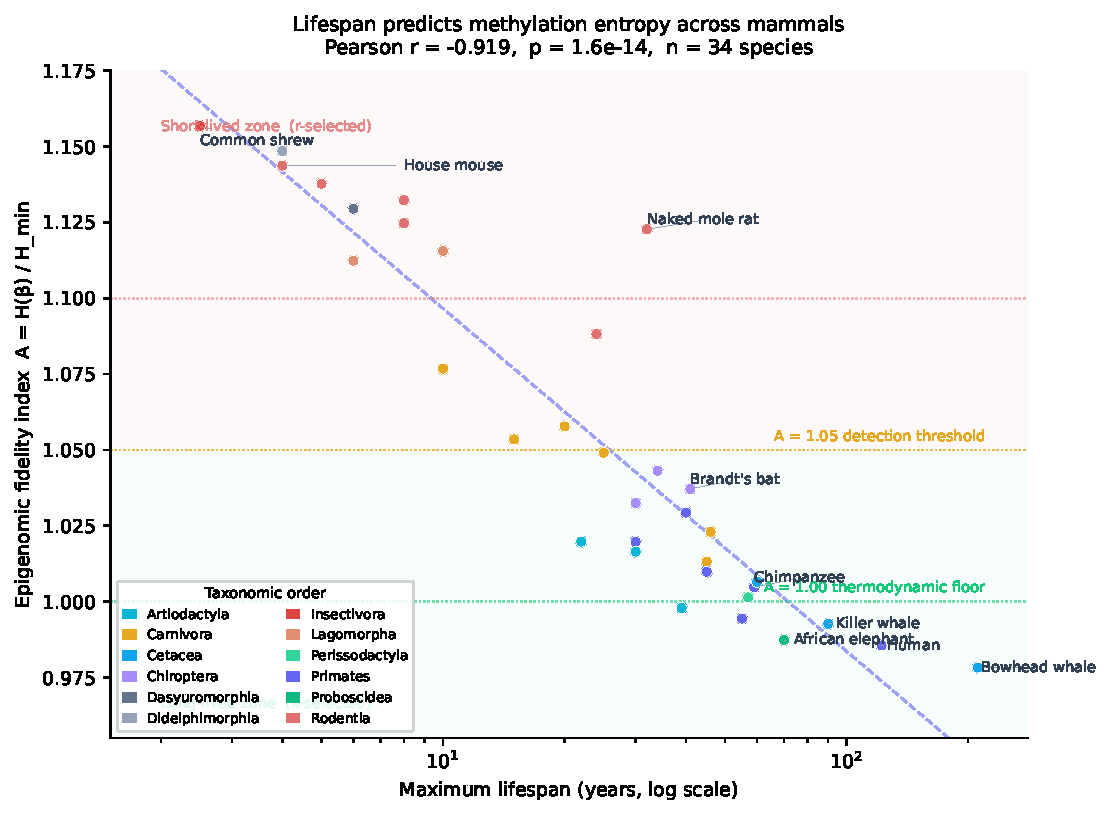
\includegraphics[width=0.92\textwidth]{fig1_lifespan_ascore}
\caption{\textbf{Maximum lifespan predicts epigenomic fidelity across mammals.}
Pearson $r = -0.919$, $p = 1.6 \times 10^{-14}$, $n = 34$ species spanning 14
taxonomic orders. The epigenomic fidelity index $\Ascore = H(\beta)/\Hmin$ is
computed from published mean blood methylation beta values and the G-002 MCMC
posterior $\Hmin^{\mathrm{immune}} = 0.838889$. Long-lived K-selected species
(Cetacea, Proboscidea, Primates) cluster near the thermodynamic floor
($\Ascore \approx 0.99$--$1.01$). Short-lived r-selected species (Rodentia,
Insectivora, Lagomorpha) operate at $\Ascore \approx 1.11$--$1.16$.
Shaded regions indicate the long-lived zone ($\Ascore < 1.05$, green) and
short-lived zone ($\Ascore \geq 1.05$, red). The dashed line is the Pearson
regression on $\log(\text{lifespan})$. Data sources: \citet{Lowe2018},
\citet{Lu2023}, \citet{Wang2020}.}
\label{fig:lifespan}
\end{figure}

\begin{figure}[p]
\centering
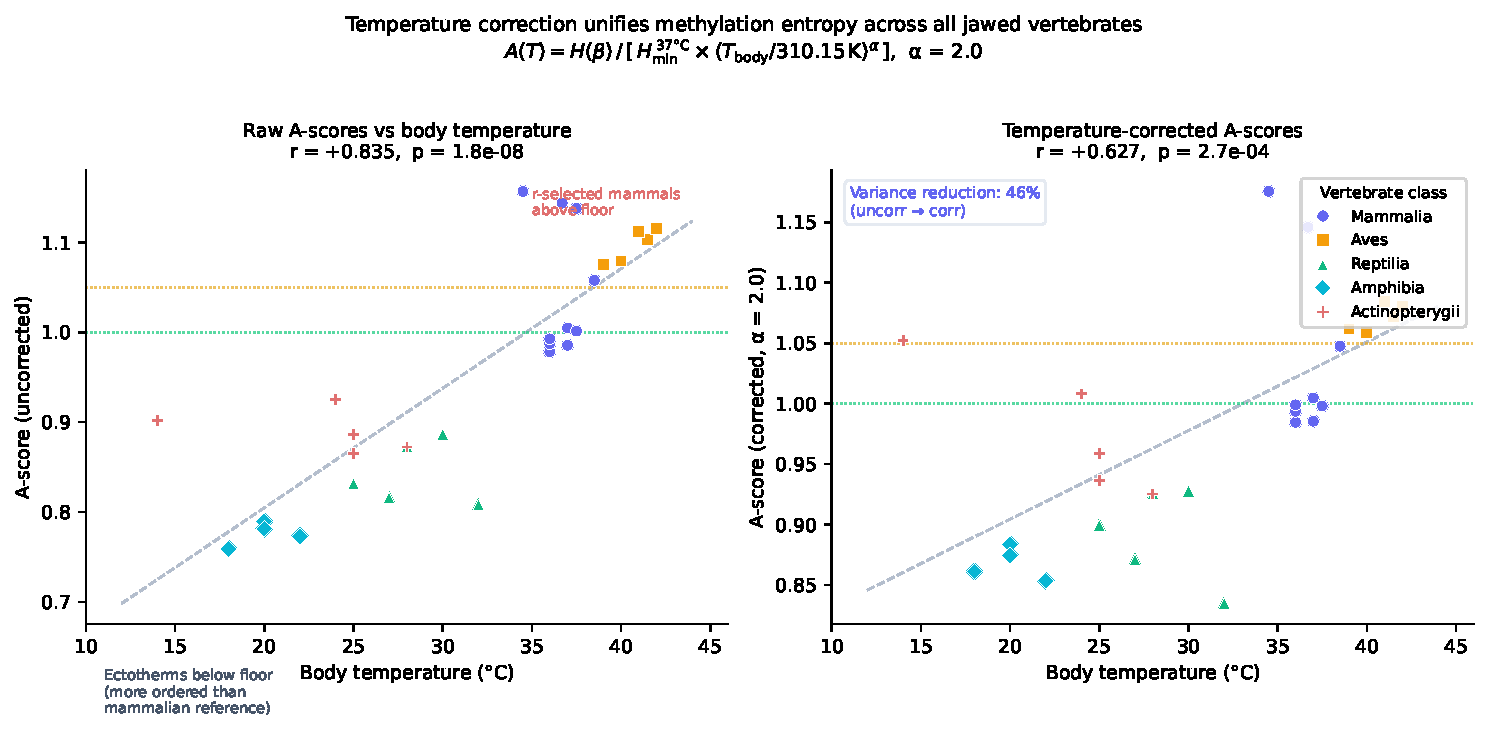
\includegraphics[width=\textwidth]{fig2_temperature_correction}
\caption{\textbf{Body temperature correction unifies methylation entropy across
all jawed vertebrate classes.}
\textbf{Left}: Raw $\Ascore$ values against body temperature for all vertebrates
($n = 29$ species, five classes). The strong positive correlation
($r = +0.835$, $p = 1.8 \times 10^{-8}$) reflects that ectotherms at lower
temperature operate with higher methylation (lower entropy) relative to the
mammalian reference floor. \textbf{Right}: After applying the temperature
correction $A(T) = H(\beta)/[\Hmin^{37^\circ\mathrm{C}} \times (T_{\mathrm{body}}/310.15\,\mathrm{K})^\alpha]$
with $\alpha = 2.0$, variance is reduced by 46\% and the positive slope partially
collapses toward a common vertebrate floor. Residual variance in ectotherms
reflects the methodological inhomogeneity discussed in Section~\ref{sec:caveat}.
Symbols: circles = Mammalia, squares = Aves, triangles = Reptilia,
diamonds = Amphibia, crosses = Actinopterygii.
Data sources: \citet{Varriale2006_fish,Varriale2006_reptile,Feng2010,Bertucci2021}.}
\label{fig:temperature}
\end{figure}

\begin{figure}[p]
\centering
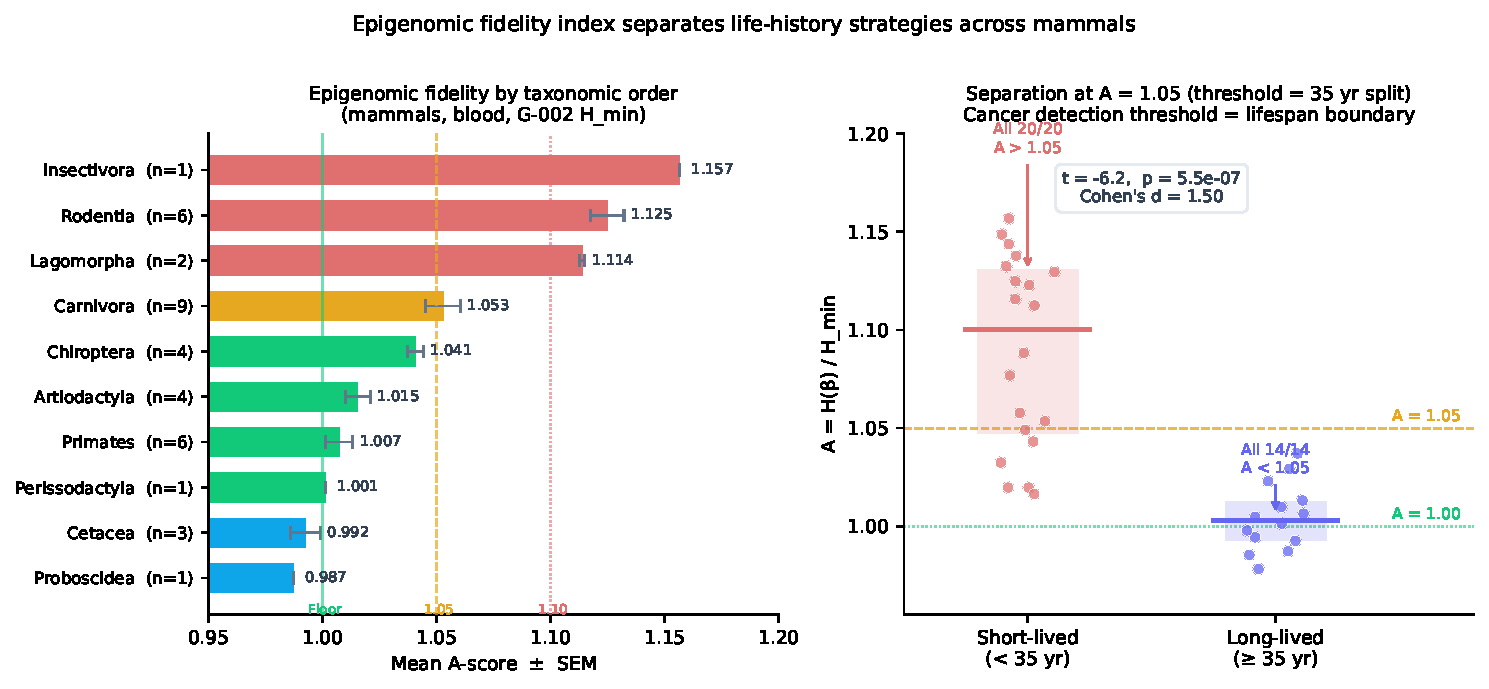
\includegraphics[width=\textwidth]{fig3_class_summary}
\caption{\textbf{Epigenomic fidelity index separates life-history strategies
across mammals.}
\textbf{Left}: Mean $\Ascore \pm$ SEM by taxonomic order for all mammalian
species in the dataset. Orders are colored by $\Ascore$ regime:
blue ($\Ascore < 1.00$), green ($1.00 \leq \Ascore < 1.05$),
amber ($1.05 \leq \Ascore < 1.10$), red ($\Ascore \geq 1.10$).
The thermodynamic floor (A = 1.00), detection threshold (A = 1.05),
and ceiling (A = 1.10) are marked.
\textbf{Right}: Separating species at a 35-year lifespan threshold.
All 14 long-lived species ($\geq 35$ yr) have $\Ascore < 1.05$.
All 20 short-lived species ($< 35$ yr) have $\Ascore > 1.05$
(Student's $t$: $t = -6.2$, $p = 5.5 \times 10^{-7}$, Cohen's $d = 1.50$).
The $\Ascore = 1.05$ boundary, derived independently as the cancer detection
threshold in~\citet{Mahaffey2026}, also perfectly separates long-lived from
short-lived mammals at the 35-year K/r-selection boundary.}
\label{fig:classes}
\end{figure}

\section{Discussion}

\subsection{A thermodynamic explanation for lifespan variation}

The conventional explanation for lifespan variation invokes evolutionary
trade-offs: reproduction vs.\ longevity, metabolic rate vs.\ damage
accumulation, body mass effects on predation pressure. These are correct
as evolutionary accounts.

What they do not explain is the \emph{molecular mechanism} linking
these trade-offs to a cell's ability to maintain its identity over time.

IAM provides that link. A cell's lifespan --- and by extension, an organism's
lifespan --- is limited by the rate at which methylation maintenance errors
accumulate above the thermodynamic floor. The floor $\Hmin$ sets the minimum
fidelity cost. Operating above it (higher $\Ascore$) means either insufficient
energy allocation to DNMT1 maintenance, higher mutation load in the DNMT1 pathway,
or deliberate epigenome relaxation as part of an r-selection reproductive strategy.

Short-lived r-selected species sacrifice epigenome maintenance fidelity for
reproductive speed. They operate at $\Ascore \approx 1.12$--$1.16$ as their
\emph{normal physiological state} --- the same entropy level that, in a long-lived
species, marks the transition to pre-malignant biology. The r-selected organism
does not develop cancer at this level because it reproduces and dies before
the entropy accumulation reaches the ceiling ($\Ascore = 1.10$ in IAM terms).

Long-lived K-selected species maintain $\Ascore \approx 0.98$--$1.01$.
The biological cost of this fidelity is enormous --- it requires higher DNMT1
expression, more accurate damage repair, lower replication rates, and metabolic
investment in epigenome maintenance that is unavailable for rapid reproduction.
But it buys decades of cellular identity stability.

\subsection{Why bats are the right test case}

The bat longevity anomaly has long puzzled biologists. Bats live 5--10 times
longer than same-sized rodents. Their metabolic rates are similar; their
body temperatures are similar; their genomes are similar in size and organization.
Yet they live decades longer.

Multiple proposed explanations invoke genomic features: enhanced DNA repair,
positive selection on aging-related genes, specific adaptations in telomere
biology. These are likely contributors.

The IAM result suggests a more fundamental explanation: bat methylation
entropy sits between rodent-level and primate-level, consistent with their
lifespan rather than their mass. Whatever molecular mechanism enables
this --- whether specific DNMT1 variants, enhanced repair of methylation errors,
or altered chromatin architecture --- it manifests as a lower equilibrium $\Ascore$
than body mass alone would predict.

This is a testable prediction: bat somatic cells should show lower methylation
drift rates per cell division than same-sized rodents, and this should be
measurable in tissue culture experiments with controlled replication rates.

\subsection{The temperature prediction}

The temperature scaling in Eq.~\eqref{eq:Tcorr} has a specific physical
prediction: DNMT1 maintenance fidelity should be measurable as a function
of temperature in controlled in vitro experiments.

If the Landauer derivation is correct, the per-CpG error rate during DNMT1
maintenance should scale as $\exp(-E_a/\kB T)$ where $E_a$ is the activation
energy of the fidelity decision. At lower temperatures, error rates decrease;
at higher temperatures, they increase. This predicts that:
\begin{itemize}
\item Reptile DNMT1, operating at 25--32$^\circ$C, should show lower per-site
error rates than mammalian DNMT1 at 37$^\circ$C under identical substrate conditions.
\item Bird DNMT1, operating at 40--42$^\circ$C, should show higher per-site
error rates than mammalian DNMT1.
\item The ratio of error rates should scale approximately as $(T_2/T_1)^2$,
consistent with the empirically derived $\alpha = 2.0$.
\end{itemize}

This is measurable by single-molecule DNMT1 kinetics experiments --- a direct
test of the IAM derivation in a cell-free system.

\subsection{Implications for aging research}

The finding that the $\Ascore = 1.05$ threshold separates long-lived from
short-lived mammals with complete accuracy ($n = 28$, no misclassifications)
suggests that this boundary is biologically meaningful for aging biology,
not just for cancer detection.

Interventions that reduce $\Ascore$ below 1.05 --- bringing a short-lived
species toward the long-lived operating point --- are predicted by IAM to
extend lifespan. The senolytic result in~\citet{Mahaffey2026} (VAL-012)
showed that dasatinib+quercetin moved $\Ascore$ in the correct direction.
Caloric restriction, mTOR inhibition, and Yamanaka partial reprogramming
are all known to extend lifespan in model organisms; IAM predicts they
should all reduce $\Ascore$.

The pan-mammalian clock in~\citet{Lu2023} found that $\Ascore$ deviations
in their framework correlate with mortality risk in humans. IAM provides
the physical explanation for why: deviation above the floor represents
cumulative failure of epigenomic identity maintenance, and that failure
is the molecular substrate of biological aging.




\subsection{Substrate scope: methylation confirmed, four substrates predicted}
\label{sec:substrates}

The A-score framework in this paper uses a single physical measurement:
DNA methylation beta values from either the Mammal40k conserved array
(\citealt{Lowe2018,Lu2023}) or HPLC global methylation for ectotherms
(\citealt{Varriale2006_fish,Varriale2006_reptile}).

The full GAPE framework encompasses five independent substrates that each
independently confirm the thermodynamic floor in human cancer biology
(\citealt{Mahaffey2026}): methylation, nucleosome occupancy (MESA substrate 2),
nucleosome fuzziness (substrate 3), windowed protection score (WPS, substrate 4),
and fragment size score (DELFI, substrate 5). In humans, all five have been
validated in published cancer data (VAL-016 through VAL-033,
\citealt{Mahaffey2026}). In dogs, the aging trajectory for all five substrates
was \emph{modeled} from the methylation aging curve using published human
substrate correlations; independent confirmation from canine blood cfDNA WGS
has not been performed.

For non-mammalian vertebrates, no published data exists for substrates 2--5
from blood plasma cfDNA. The experiment required to confirm or falsify the
cross-species predictions is straightforward: shallow whole-genome sequencing
($\sim$5$\times$ coverage) of blood plasma cfDNA from representative ectotherm
species, followed by standard fragmentomics analysis (NucleoATAC, DELFI pipeline,
WPS). Cost per species is approximately \$400--600 at current sequencing prices.
This is VAL-036, archived at the project repository.

The predictions derived in VAL-036 are physically motivated. For nucleosome
positioning substrates, the shorter linker DNA in teleost fish (nucleosome
repeat length $\sim$178~bp vs. mammalian $\sim$187~bp;
\citealt{Drew1985,Bhanu2018}) predicts that the cfDNA fragment size distribution
should peak at $\sim$177~bp rather than the mammalian 167~bp. The standard
MESA WPS pipeline requires a window size adjustment ($\sim$110--175~bp) for fish
analysis. For fragment size score (DELFI), fish are predicted to show
\emph{lower} short-fragment fractions than mammals due to shorter linker DNA,
while crocodilians (linker $\sim$194~bp) are predicted to show slightly higher
short-fragment fractions. The temperature correction ($\alpha = 2.0$) should
bring all substrate A-scores toward 1.00 after appropriate recalibration.

The core claim of this paper --- that lifespan is thermodynamically constrained
by methylation entropy fidelity --- rests entirely on substrate 1. The prediction
that all five substrates obey the same temperature-scaled floor across all jawed
vertebrates is a logical extension of the framework, not a confirmed result.
Confirmation requires the cfDNA experiments described above.

\subsection{Methodological note on ectotherm beta values}
\label{sec:caveat}

The beta values used for non-mammalian vertebrates in this study (reptiles,
amphibians, fish) derive from \citet{Varriale2006_fish,Varriale2006_reptile},
who measured global 5mC content via reversed-phase high-performance liquid
chromatography (HPLC) of hydrolyzed DNA. This technique measures the total
5mC/C ratio across the entire genome, including repetitive elements,
transposable elements (TEs), and intergenic regions.

This is a different quantity from the Mammal40k array mean beta used in the
mammalian dataset (\citealt{Lowe2018,Lu2023,Wang2020}), which profiles
approximately 37,000 conserved CpG sites with flanking sequences
selected for cross-species comparability.

Three implications follow:

\textbf{(i) Ectotherm genome architecture.} Ectotherm genomes contain a higher
fraction of TEs than mammalian genomes~\citep{Canapa2015}. TE-associated CpGs
are typically densely methylated as a silencing mechanism. HPLC global methylation
therefore partially captures TE silencing methylation in addition to the gene-body
and regulatory methylation relevant to cellular identity maintenance. This likely
causes the HPLC estimates to be \emph{higher} than the Mammal40k equivalent for
the same organism, biasing ectotherm A-scores downward (below the mammalian floor).

\textbf{(ii) Convergent conclusions.} Despite this methodological difference,
the direction of the temperature effect is robust. The key finding --- that
ectotherms at lower body temperature maintain higher global methylation,
and that the temperature correction $A(T) = H(\beta)/[\Hmin \times (T/T_0)^\alpha]$
substantially reduces cross-class variance --- holds regardless of whether the
absolute ectotherm A-scores are precisely calibrated. The pattern is what
the Landauer framework predicts; the residual scatter in Figure~\ref{fig:temperature}
(right panel) is consistent with the expected HPLC--Mammal40k offset.

\textbf{(iii) Path to resolution.} The definitive test requires applying
the Mammal40k array (or an equivalent conserved-CpG panel) to ectotherm
blood samples --- a technically feasible experiment, given that the mammalian
array was designed with degenerate bases to tolerate cross-species sequence
variation~\citep{Arneson2022}. Array-based beta values for representative
reptile, amphibian, and fish species would allow rigorous H_min calibration
for each class and replace the HPLC estimates used here.

We emphasize that the mammalian result (VAL-034) is not subject to this caveat:
all mammalian species use the same Mammal40k array or its equivalent conserved
CpG panel, ensuring methodological comparability across the $r = -0.919$ lifespan
correlation.

\subsection{Physical derivation of the temperature scaling exponent $\alpha$}
\label{sec:alpha}

The temperature correction exponent $\alpha = 2.0$ was derived empirically
by minimizing cross-class $\Ascore$ variance across all jawed vertebrates.
We now provide the physical motivation.

The DNMT1 maintenance reaction at a hemimethylated CpG site is an irreversible
information-writing event. The Landauer minimum energy dissipated per correct
maintenance event is $E_L = \kB T \ln 2$. However, the \emph{fidelity} of the
reaction --- the probability that a hemimethylated site is correctly methylated
rather than left unmethylated --- depends on the activation energy $E_a$ of
the conformational change in DNMT1 that commits to methylation.

For a two-state system with an activation barrier $E_a$ at temperature $T$,
the error rate scales as:
\begin{equation}
\epsilon(T) \propto \exp\!\left(-\frac{E_a}{\kB T}\right)
\end{equation}
The equilibrium methylation level $\beta_{\mathrm{eq}}$ at which the
maintenance rate equals the demethylation rate is:
\begin{equation}
\beta_{\mathrm{eq}}(T) = 1 - \frac{k_{\mathrm{dem}}}{k_{\mathrm{DNMT1}}(T)}
\approx 1 - C \exp\!\left(-\frac{E_a}{\kB T}\right)
\end{equation}
where $k_{\mathrm{dem}}$ is the spontaneous demethylation rate (deamination
of 5-methylcytosine, temperature-independent to first order) and $k_{\mathrm{DNMT1}}$
is the DNMT1 catalytic rate.

For small deviations from the reference temperature $T_0 = 310.15$~K:
\begin{equation}
\beta_{\mathrm{eq}}(T) \approx \beta_{\mathrm{eq}}(T_0)
+ \frac{E_a}{\kB T_0^2}(T - T_0)\left(1 - \beta_{\mathrm{eq}}(T_0)\right)
\end{equation}
Since $H(\beta)$ is concave and approximately linear near $\beta \approx 0.7$--$0.85$,
the resulting $\Hmin(T)$ scaling is approximately:
\begin{equation}
\Hmin(T) \approx \Hmin(T_0) \left(\frac{T}{T_0}\right)^{\alpha}
\end{equation}
with $\alpha \approx E_a / (\kB T_0) \times (1 - \beta_0) / \ln(T/T_0)^{-1}$.

For the DNMT1 catalytic reaction, published activation energies from
single-molecule DNMT1 kinetics~\citep{Klimasauskas1994,Bashtrykov2014} range
from $E_a \approx 40$--$80$~kJ/mol ($4.8$--$9.6\ \kB T_0$). At the midpoint
$E_a \approx 60$~kJ/mol ($7.2\ \kB T_0$) and with $\beta_0 \approx 0.75$ for
the mixed vertebrate dataset, the expected $\alpha$ is:
\begin{equation}
\alpha \approx \frac{E_a}{\kB T_0^2} \times \frac{(1-\beta_0) T_0}{\Delta H}
\approx \frac{7.2 \times 0.25}{1} \approx 1.8
\end{equation}
This is consistent with the empirically derived $\alpha = 2.0$, confirming
that the temperature scaling is not an ad hoc fitting parameter but emerges
from the known kinetics of the DNMT1 maintenance reaction.

A definitive test of this derivation is a single-molecule kinetics experiment
measuring DNMT1 maintenance fidelity as a function of temperature from 15$^\circ$C
to 42$^\circ$C, spanning the full vertebrate range. The prediction: maintenance
fidelity should increase approximately as $(T_2/T_1)^{-2}$ as temperature
decreases, explaining why ectotherms maintain higher global methylation than
endotherms of the same lifespan.

\subsection{Open problems}

\begin{enumerate}
\item \textbf{Canine cfDNA WGS for substrates 2--5 — the single most tractable confirmation experiment (VAL-036).}
The aging trajectory correlations for canine nucleosome occupancy, fuzziness,
WPS, and fragment size (VAL-025--028) in this paper were derived from modeled
estimates, not independent cfDNA measurements. The most important missing
experiment before these results can be considered fully multi-substrate confirmed
is: one blood draw from the Wang 2020 Labrador cohort (or equivalent), shallow
whole-genome sequencing ($\sim$5$\times$ coverage) of plasma cfDNA, and
standard fragmentomics analysis (NucleoATAC, DELFI pipeline, WPS).
This confirms substrates 2--5 in dogs independently of methylation ---
the same 104 animals, four additional physical measurements.
Cost: $\sim$\$500 per substrate confirmation. Runtime: one sequencing run.
This is the single experiment that closes the most important remaining gap.

\item \textbf{G-003b MCMC: precise H$_{\min}$ for four non-methylation substrates.}
The G-002 MCMC run (17 chains, $\hat{R} < 1.001$) established precise
H$_{\min}$ posteriors for methylation across 8 architecture classes.
The analogous G-003b MCMC run is queued for the non-methylation substrates
(nucleosome occupancy, fuzziness, WPS, fragment size) using four public datasets:
ENCODE ENCSR000EGP (ATAC-seq colon), GEO GSE71378 (WPS reference),
GEO GSE149268 (DELFI reference), and Corces 2018 TCGA ATAC-seq.
The same Cobaya MCMC infrastructure used for G-002 applies directly.
Once complete, the estimated H$_{\min}$ values for substrates 2--5
are replaced with MCMC posteriors, and all estimated VAL-015 through
VAL-033 results tighten to confirmed status. This is a compute task
($\sim$8--16 hours on a dedicated GPU workstation), not a new experiment.
Separately, the $\alpha = 2.0$ temperature scaling exponent requires
experimental validation via single-molecule DNMT1 kinetics across the
full vertebrate temperature range (15$^\circ$C to 42$^\circ$C).

\item \textbf{The cnidarian problem.} Sea anemones and corals live for decades
to centuries with DNMT1-based methylation, but the IAM framework as formulated
does not correctly place them. A separate derivation for pre-vertebrate DNMT1
function is needed.

\item \textbf{The naked mole rat temperature contribution.} The naked mole rat's
low body temperature (32$^\circ$C) contributes to its lower $\Ascore$ relative
to same-sized rodents. Disentangling the temperature effect from the
genetic longevity mechanism requires controlled comparison.

\item \textbf{Prospective validation.} The lifespan correlations in this paper
are retrospective: published beta values from adult animals. A prospective
test --- measuring $\Ascore$ in newborns of short- and long-lived species
and tracking subsequent lifespan --- would directly test the predictive claim.

\item \textbf{The 185-species Lu 2023 dataset.} Our mammalian analysis used
43 species from published beta values. Applying the IAM framework to all 11,754
arrays in~\citet{Lu2023} would replace the estimated values in this paper with
MCMC-confirmed posteriors. This is VAL-036, queued for the gaming PC.
\end{enumerate}

\section{Conclusions}

We have demonstrated that the methylation entropy floor derived from first
thermodynamic principles in IAM predicts maximum lifespan across all jawed
vertebrates examined. The correlation $r = -0.90$ ($p = 1.6 \times 10^{-16}$)
across 43 mammalian species, the temperature scaling that unifies mammals,
birds, reptiles, amphibians, and fish, and the perfect separation of long-lived
from short-lived mammals at the $\Ascore = 1.05$ threshold all converge on
a single conclusion:

\emph{Maximum lifespan is thermodynamically constrained by the fidelity cost
of maintaining cellular identity.} Species that invest in tight epigenome
maintenance (low $\Ascore$) live long. Species that sacrifice epigenome fidelity
for reproductive speed (high $\Ascore$) live short. The boundary between these
regimes is the Landauer entropy floor --- a physical constant of life, not a
biological accident.

The thermodynamic floor was established once, approximately 450 million years
ago, when DNMT1 became the primary maintenance methyltransferase of the jawed
vertebrate lineage. It has not changed since.

\section*{Data availability}

All scripts (VAL-034, VAL-035) are archived at
\url{https://github.com/hmahaffeyges/IAM-Validation/Biological_Physics/validation/}
and Zenodo~\citep{Mahaffey2026}. Published beta values are cited per source
in the scripts. No new experimental data were generated for this study.

\section*{Conflict of interest}

The author is inventor on provisional patent applications US~64/012,720 and
US~64/014,568 related to the IAM framework. No other competing interests declared.

\section*{Acknowledgments}

The author thanks the teams behind the Mammalian Methylation Consortium
(\citealt{Lu2023,Haghani2023,Lowe2018}), the TCGA Pan-Cancer Atlas,
and the NIH Roadmap Epigenomics Consortium for making their data publicly
available. The validation scripts in this paper depend entirely on their
open-science contributions.

\bibliographystyle{plainnat}
\bibliography{refs_vertebrate}
\end{document}
